\section{Flowcharts} \label{app_sec:flowcharts}

\subsection{Iterative Parameterization}

\subsubsection{Shafts} \label{app_subsec:shaft_flowchart}

\begin{figure}[H]
    \centering
    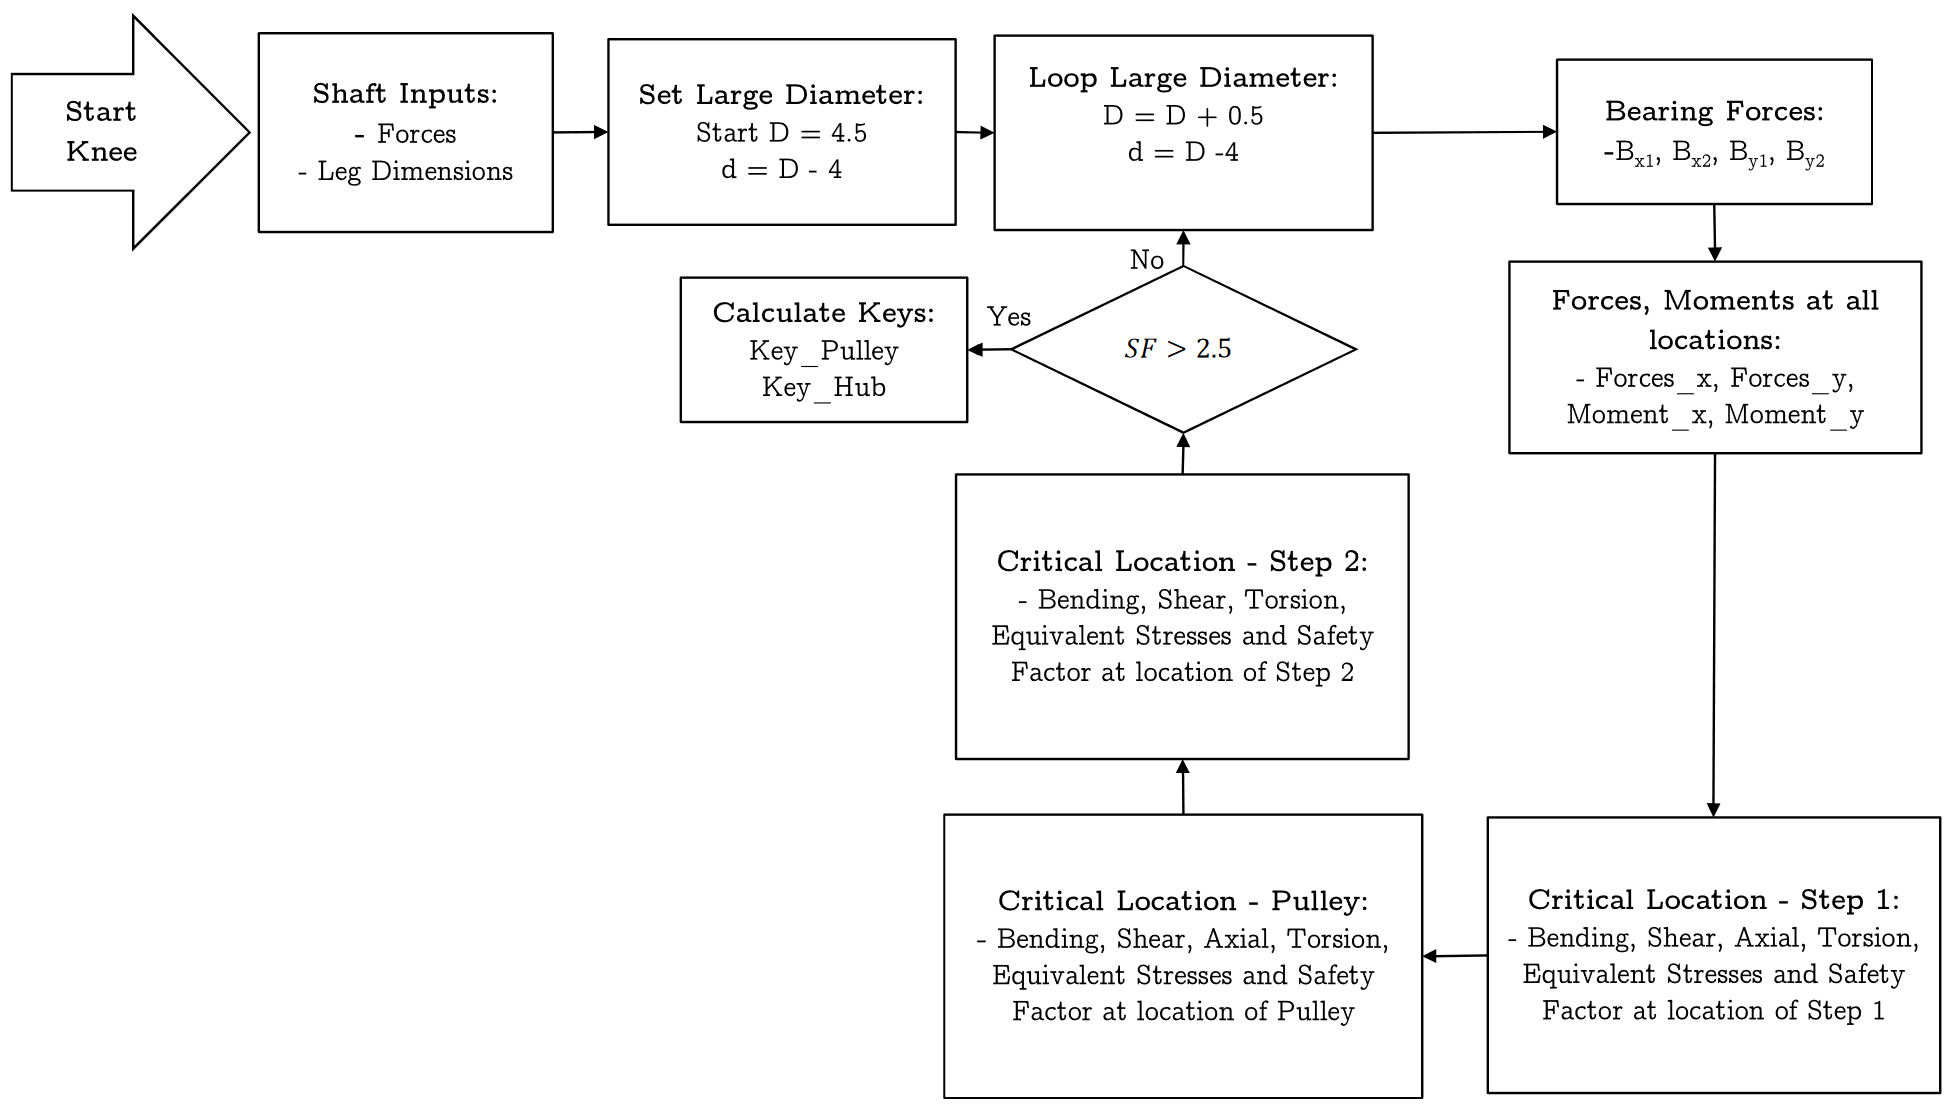
\includegraphics[width=\textwidth]{6_Appendices/Flowcharts/shaftFlowChart_Knee.png}
    \caption{Shaft Flow Chart (Knee)}
    \label{fig:shaft_flowchart(knee)}
\end{figure}{}

\begin{figure}[H]
    \centering
    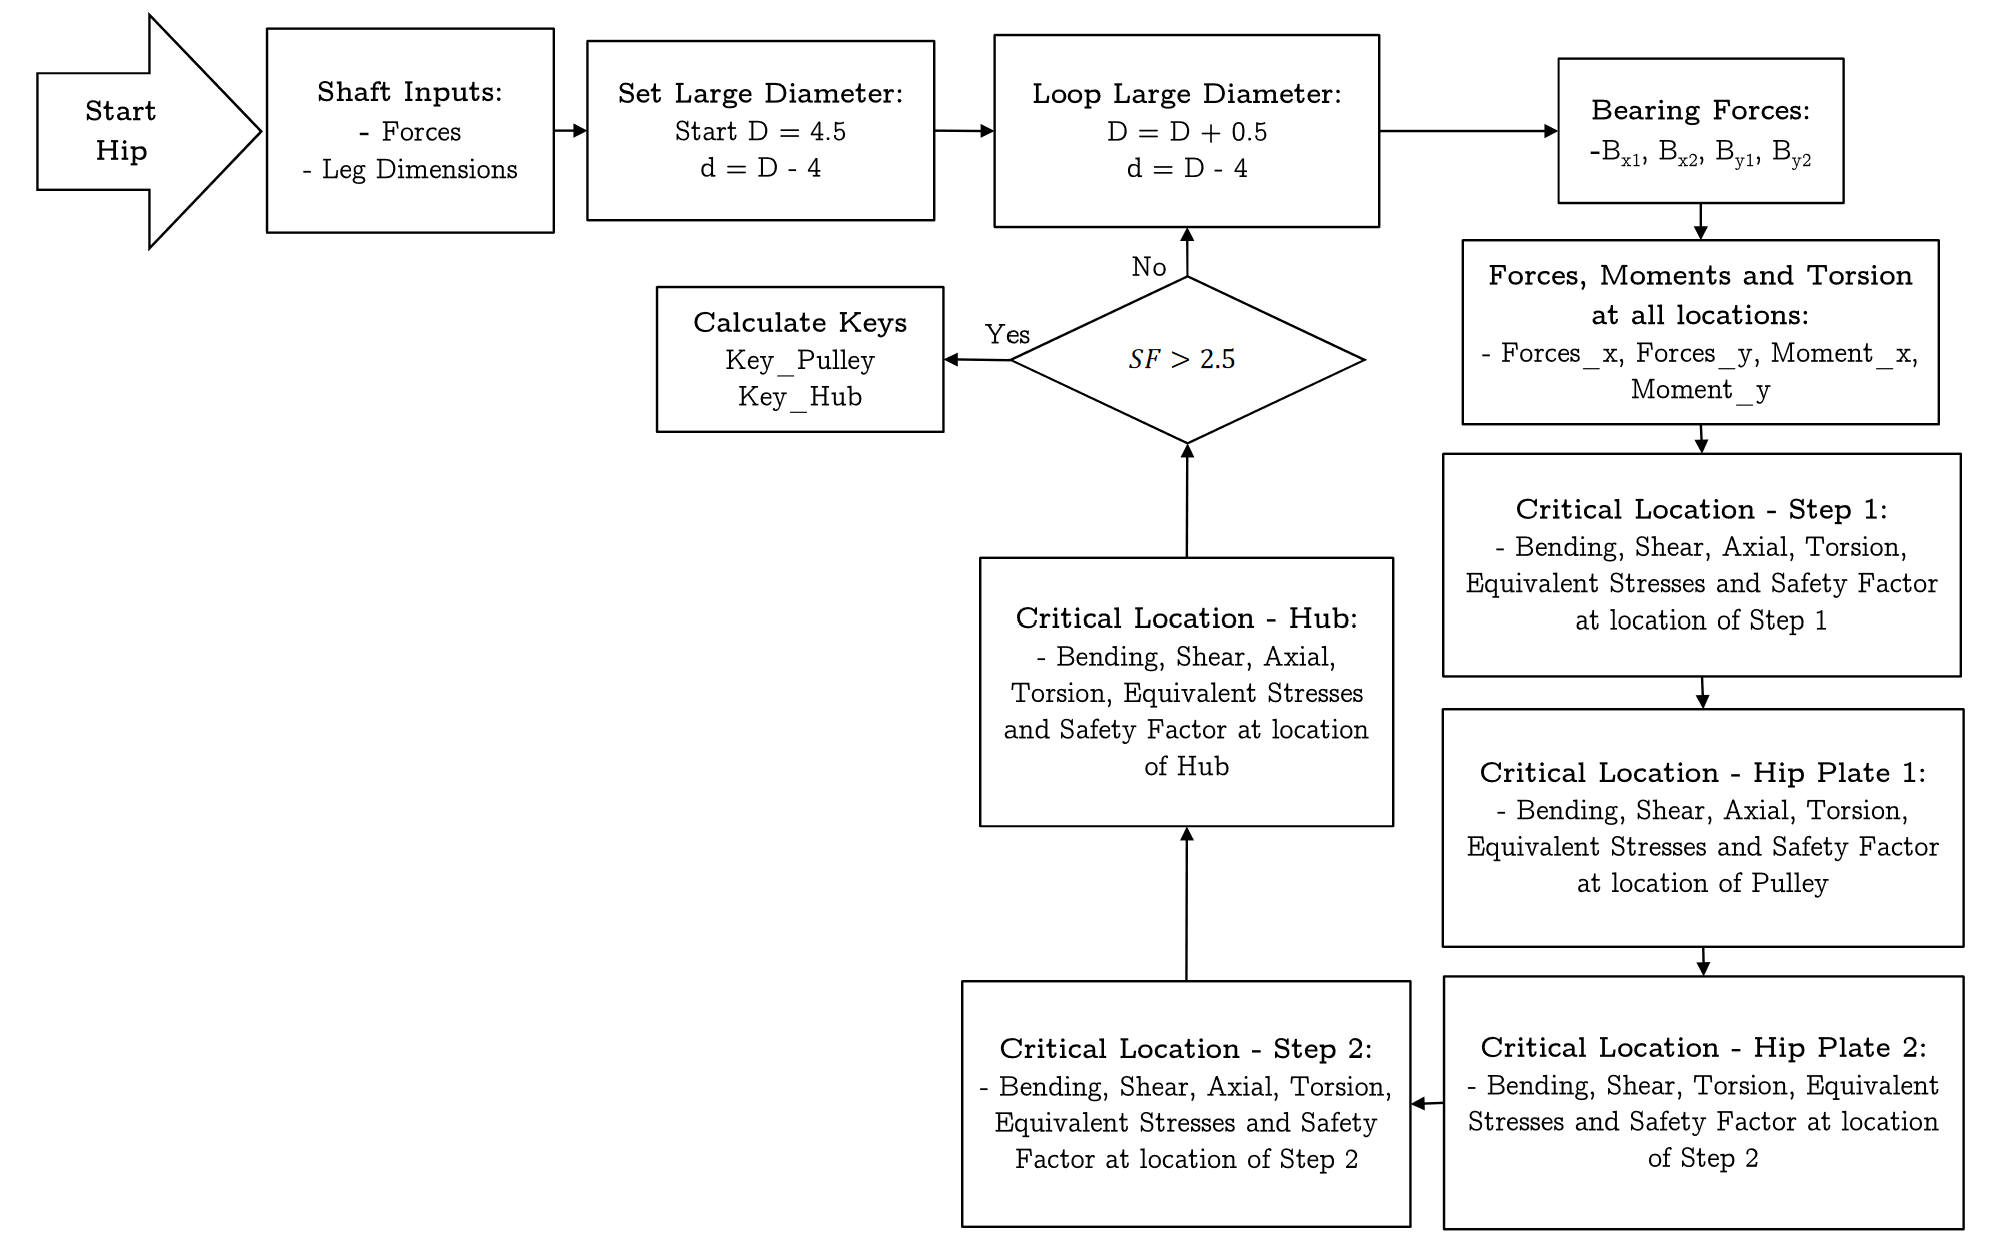
\includegraphics[width=\textwidth]{6_Appendices/Flowcharts/ShaftFlowChart_Hip.png}
    \caption{Shaft Flow Chart (Hip)}
    \label{fig:shaft_flowchart(hip)}
\end{figure}{}

\begin{figure}[H]
    \centering
    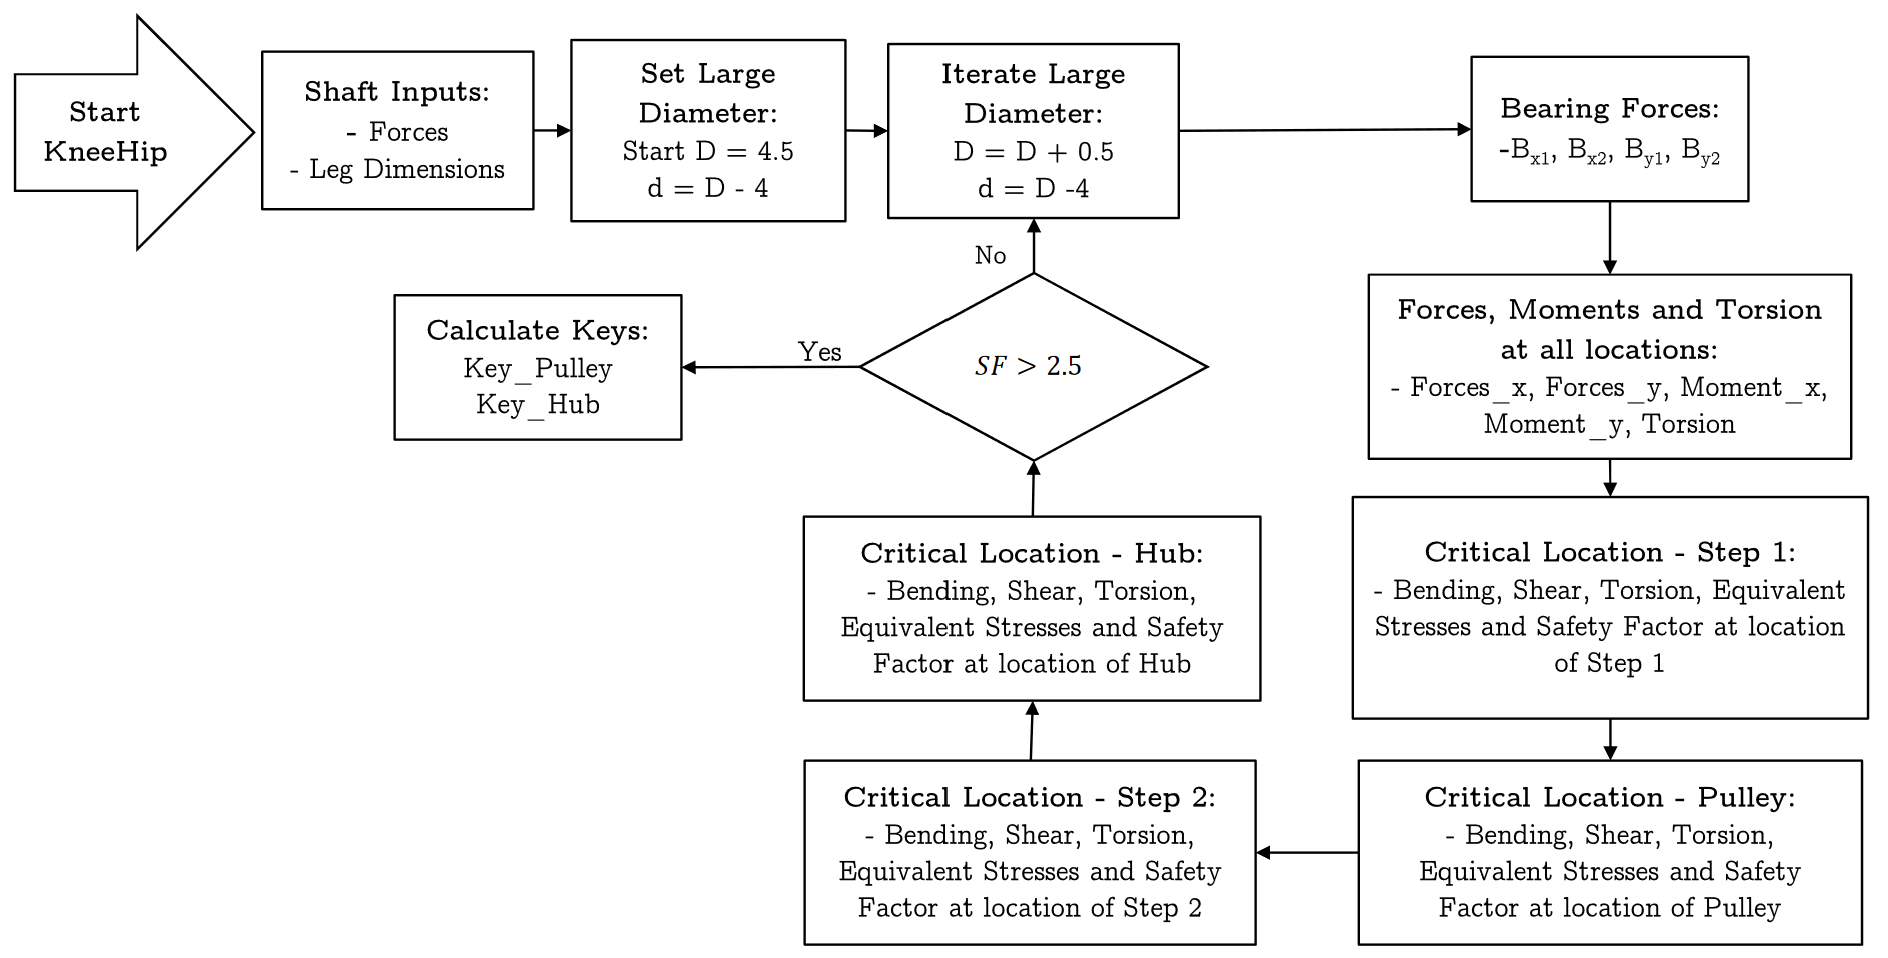
\includegraphics[width=\textwidth]{6_Appendices/Flowcharts/ShaftFlowChart_KneeHip.png}
    \caption{Shaft Flow Chart (Knee Hip)}
    \label{fig:shaft_flowchart(KneeHip)}
\end{figure}{}


\subsubsection{Belt System} \label{app_subsec:belt_flowchart}

\begin{figure}[H]
    \centering
    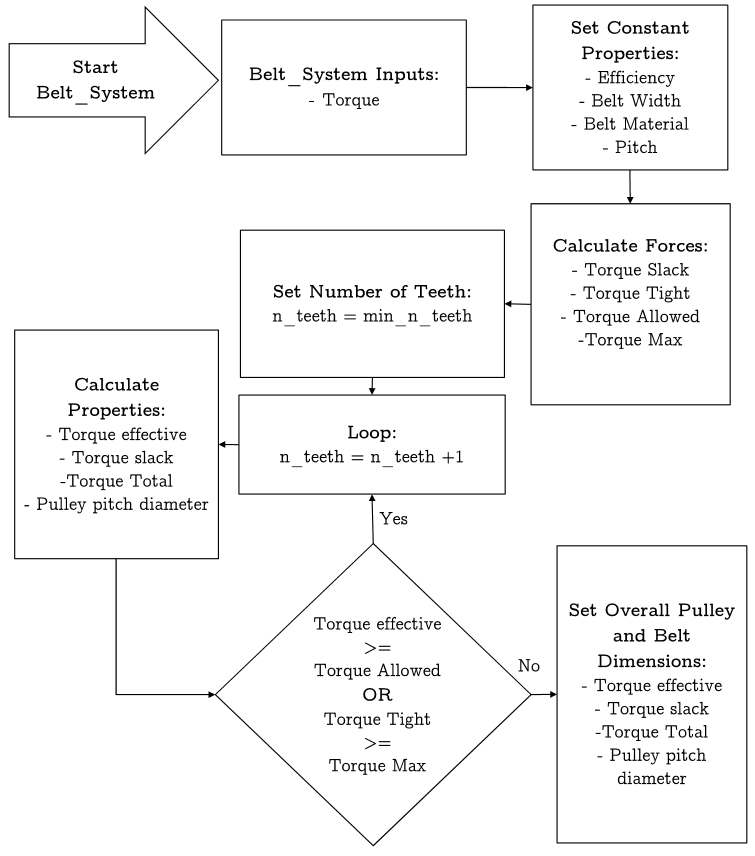
\includegraphics[width=\textwidth]{6_Appendices/Flowcharts/BeltFlowChart.png}
    \caption{Belt System Flow Chart}
    \label{fig:belt_flowchart}
\end{figure}{}


\subsubsection{Tibia Tube} \label{app_subsec:tube_flowchart}

\begin{figure}[H]
    \centering
    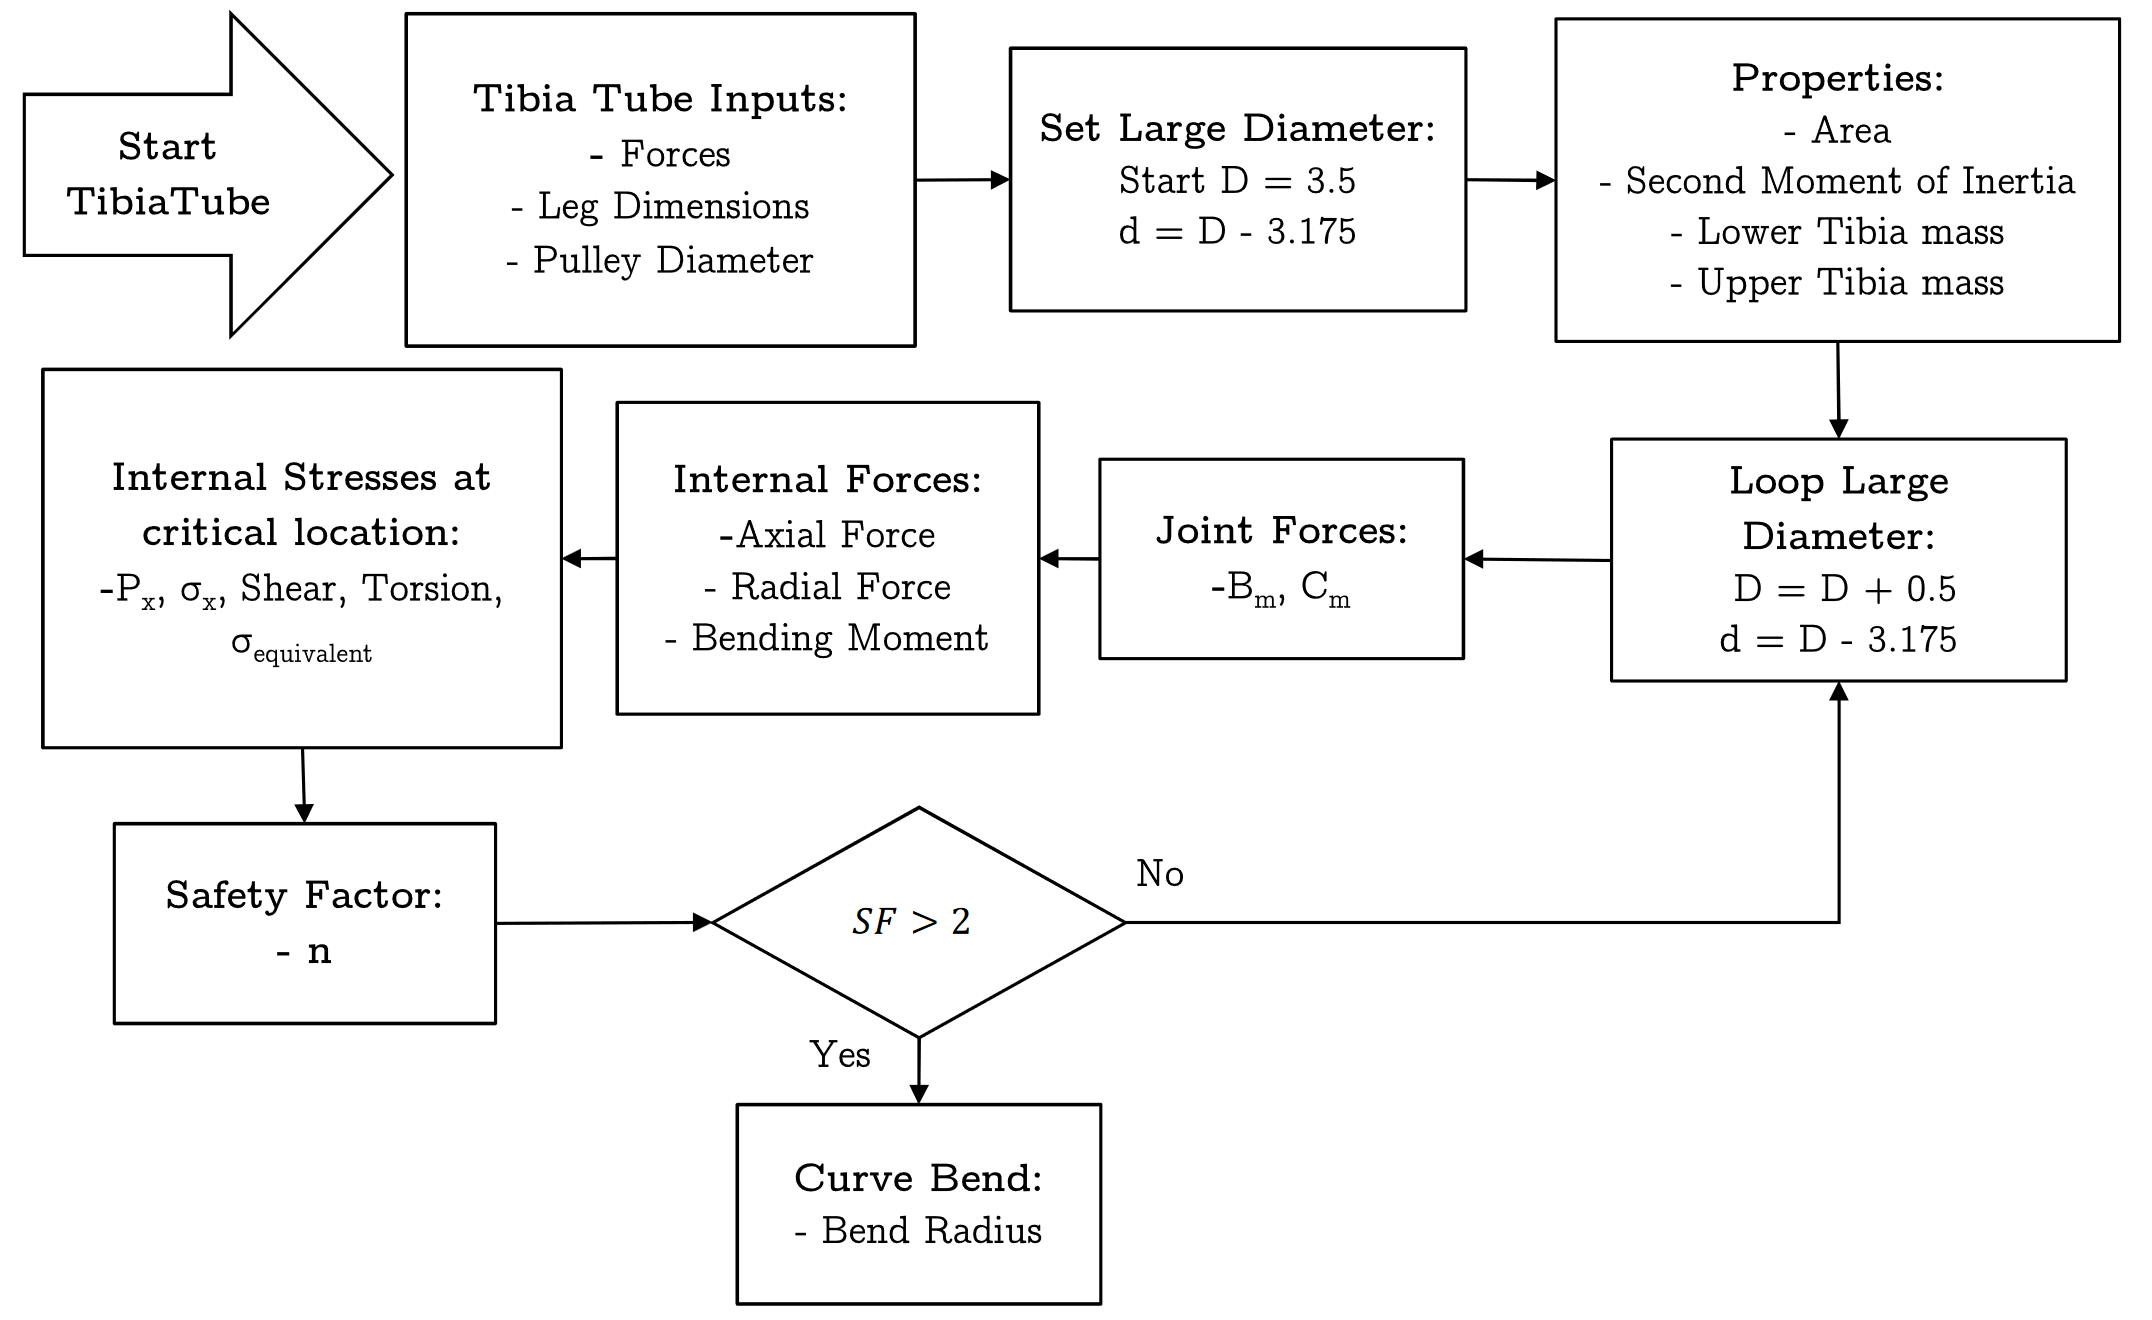
\includegraphics[width=\textwidth]{6_Appendices/Flowcharts/TibiaFlowChart.png}
    \caption{Tibia Tube Flow Chart}
    \label{fig:tube_flowchart}
\end{figure}{}

%----------- LINKAGE OPTIMIZATION -----------%
\subsection{Linkage Optimization} \label{app_sub:linkages}

The relative lengths (ratios) of the linkages $r_1$, $r_2$ and $r_3$, as well as the tibia angle $\alpha$ were set as constants in the parameterization. They were determined in Section 3.4 of the Analysis Report by generating a 3D chart of the $x$ and $y$ reach, and height from the ground $d$.
The lengths $r_1=100\text{mm}$, $r_2=50\text{mm}$, $r_3=300\text{mm}$ and $\alpha=69^{\circ}$ were originally selected to have approximately the same $x$ and $y$ reach. However, $r_2$ was increased to $120\text{mm}$ after determining that the upper tibia was too short to mount the bellow. This modified the linkage ratios slightly.
The overall workspace of the leg and the x and y reach were visualized as shown in Figure \ref{fig:workspace}.
When a user inputs the $x$ and $y$ reach, the program simply scales the linkage lengths, walking height and walking range in $x$ to match the highest value of the two inputs using the reference reaches found in \texttt{workspace.m}.
This results in the desired reach in only $x$ or $y$ being respected, with the other higher than necessary.
The relative size of the linkages has been determined experimentally and is likely far from perfect.
An ideal approach would have been to modify the lengths $r_1$, $r_2$, $r_3$, and $\alpha$ to generate a workspace that better matches both input parameters.

\begin{figure}[H]
    \centering
    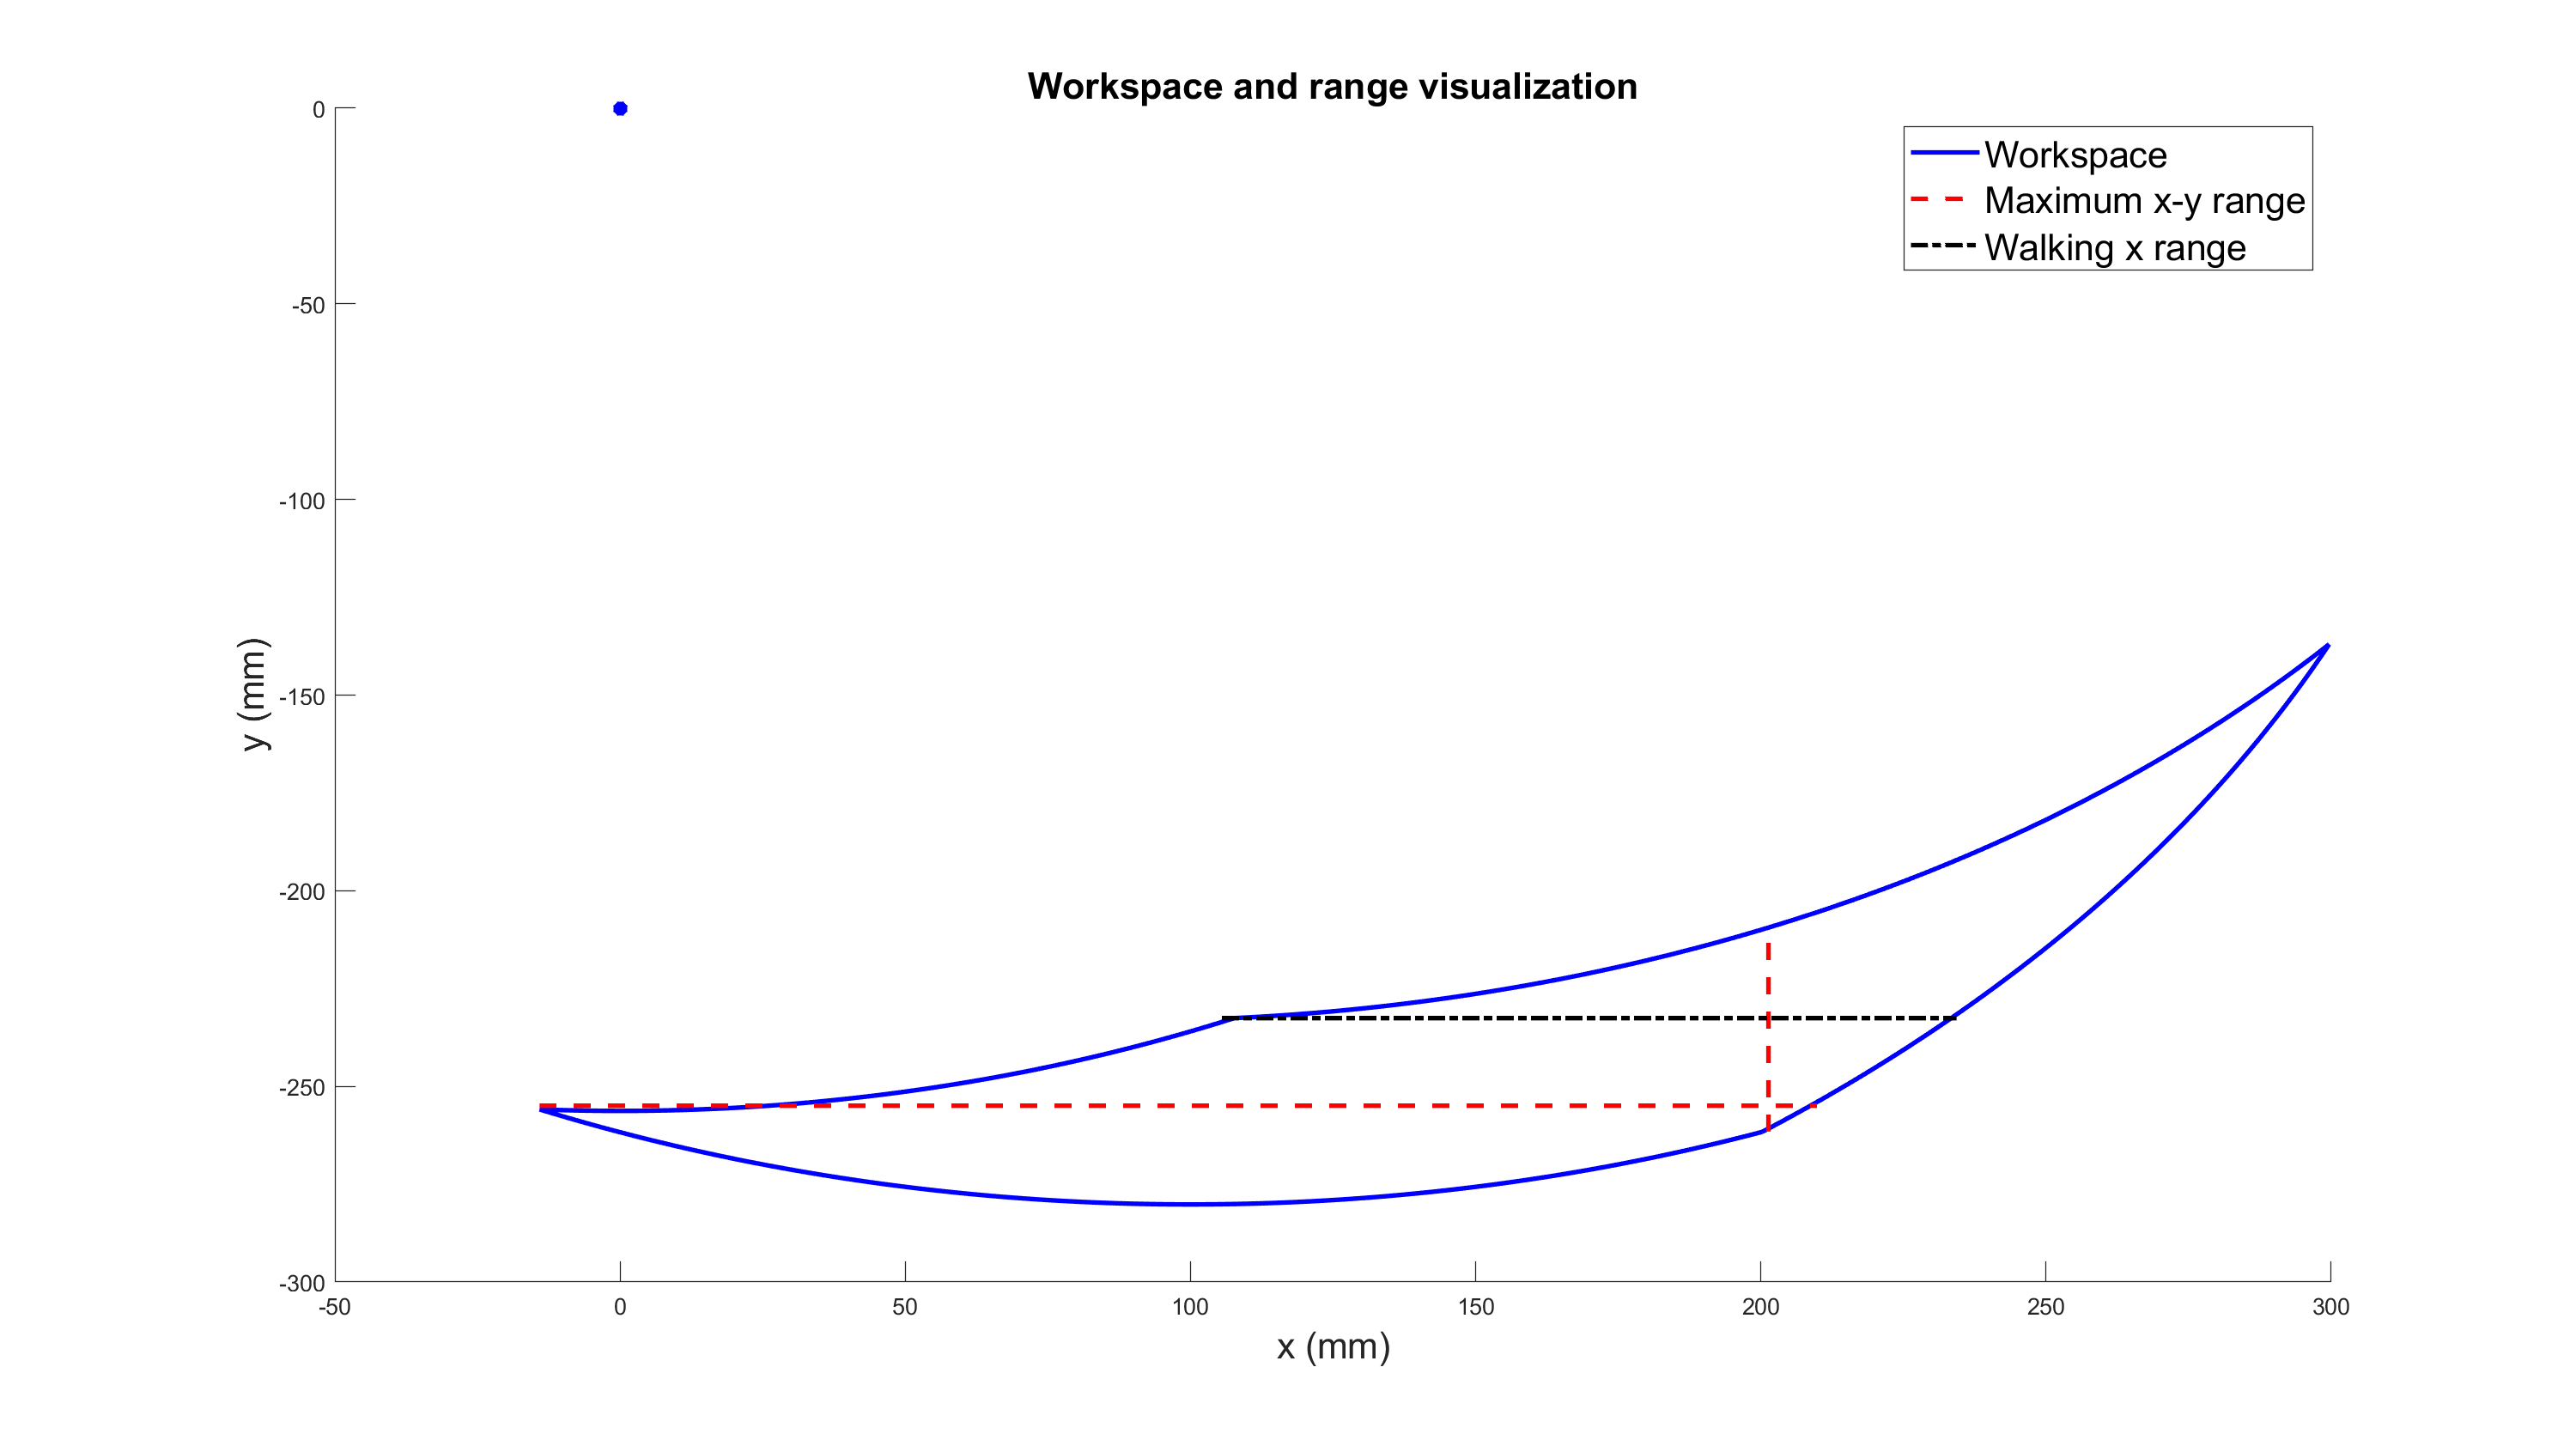
\includegraphics[width=\textwidth]{3_Parametrization/img/Workspace.png}
    \caption{Workspace visualization for $r_1=100\text{mm}$, $r_2=50\text{mm}$, $r_3=300\text{mm}$ and $\alpha=69^{\circ}$}
    \label{fig:workspace}
\end{figure}{}


\subsection{Motor and Harmonic Drive Flowcharts} \label{app_sub:HD_motor}

The motor and Harmonic Drive specs were determined by first collecting specifications for multiple sizes of motors and drives.
This data was polyfit relative to their rated torques in MATLAB and the corresponding first order polynomial coefficients $T_1$ and $T_2$ were inserted into the MATLAB files for both parts. The maximum required torque is input to the functions and all dimensions, efficiency, and other relevant specifications are output using the fit.
This procedure is outlined in Figure \ref{fig:parametrization_HD_motor}.

\begin{figure}[H]
    \centering
    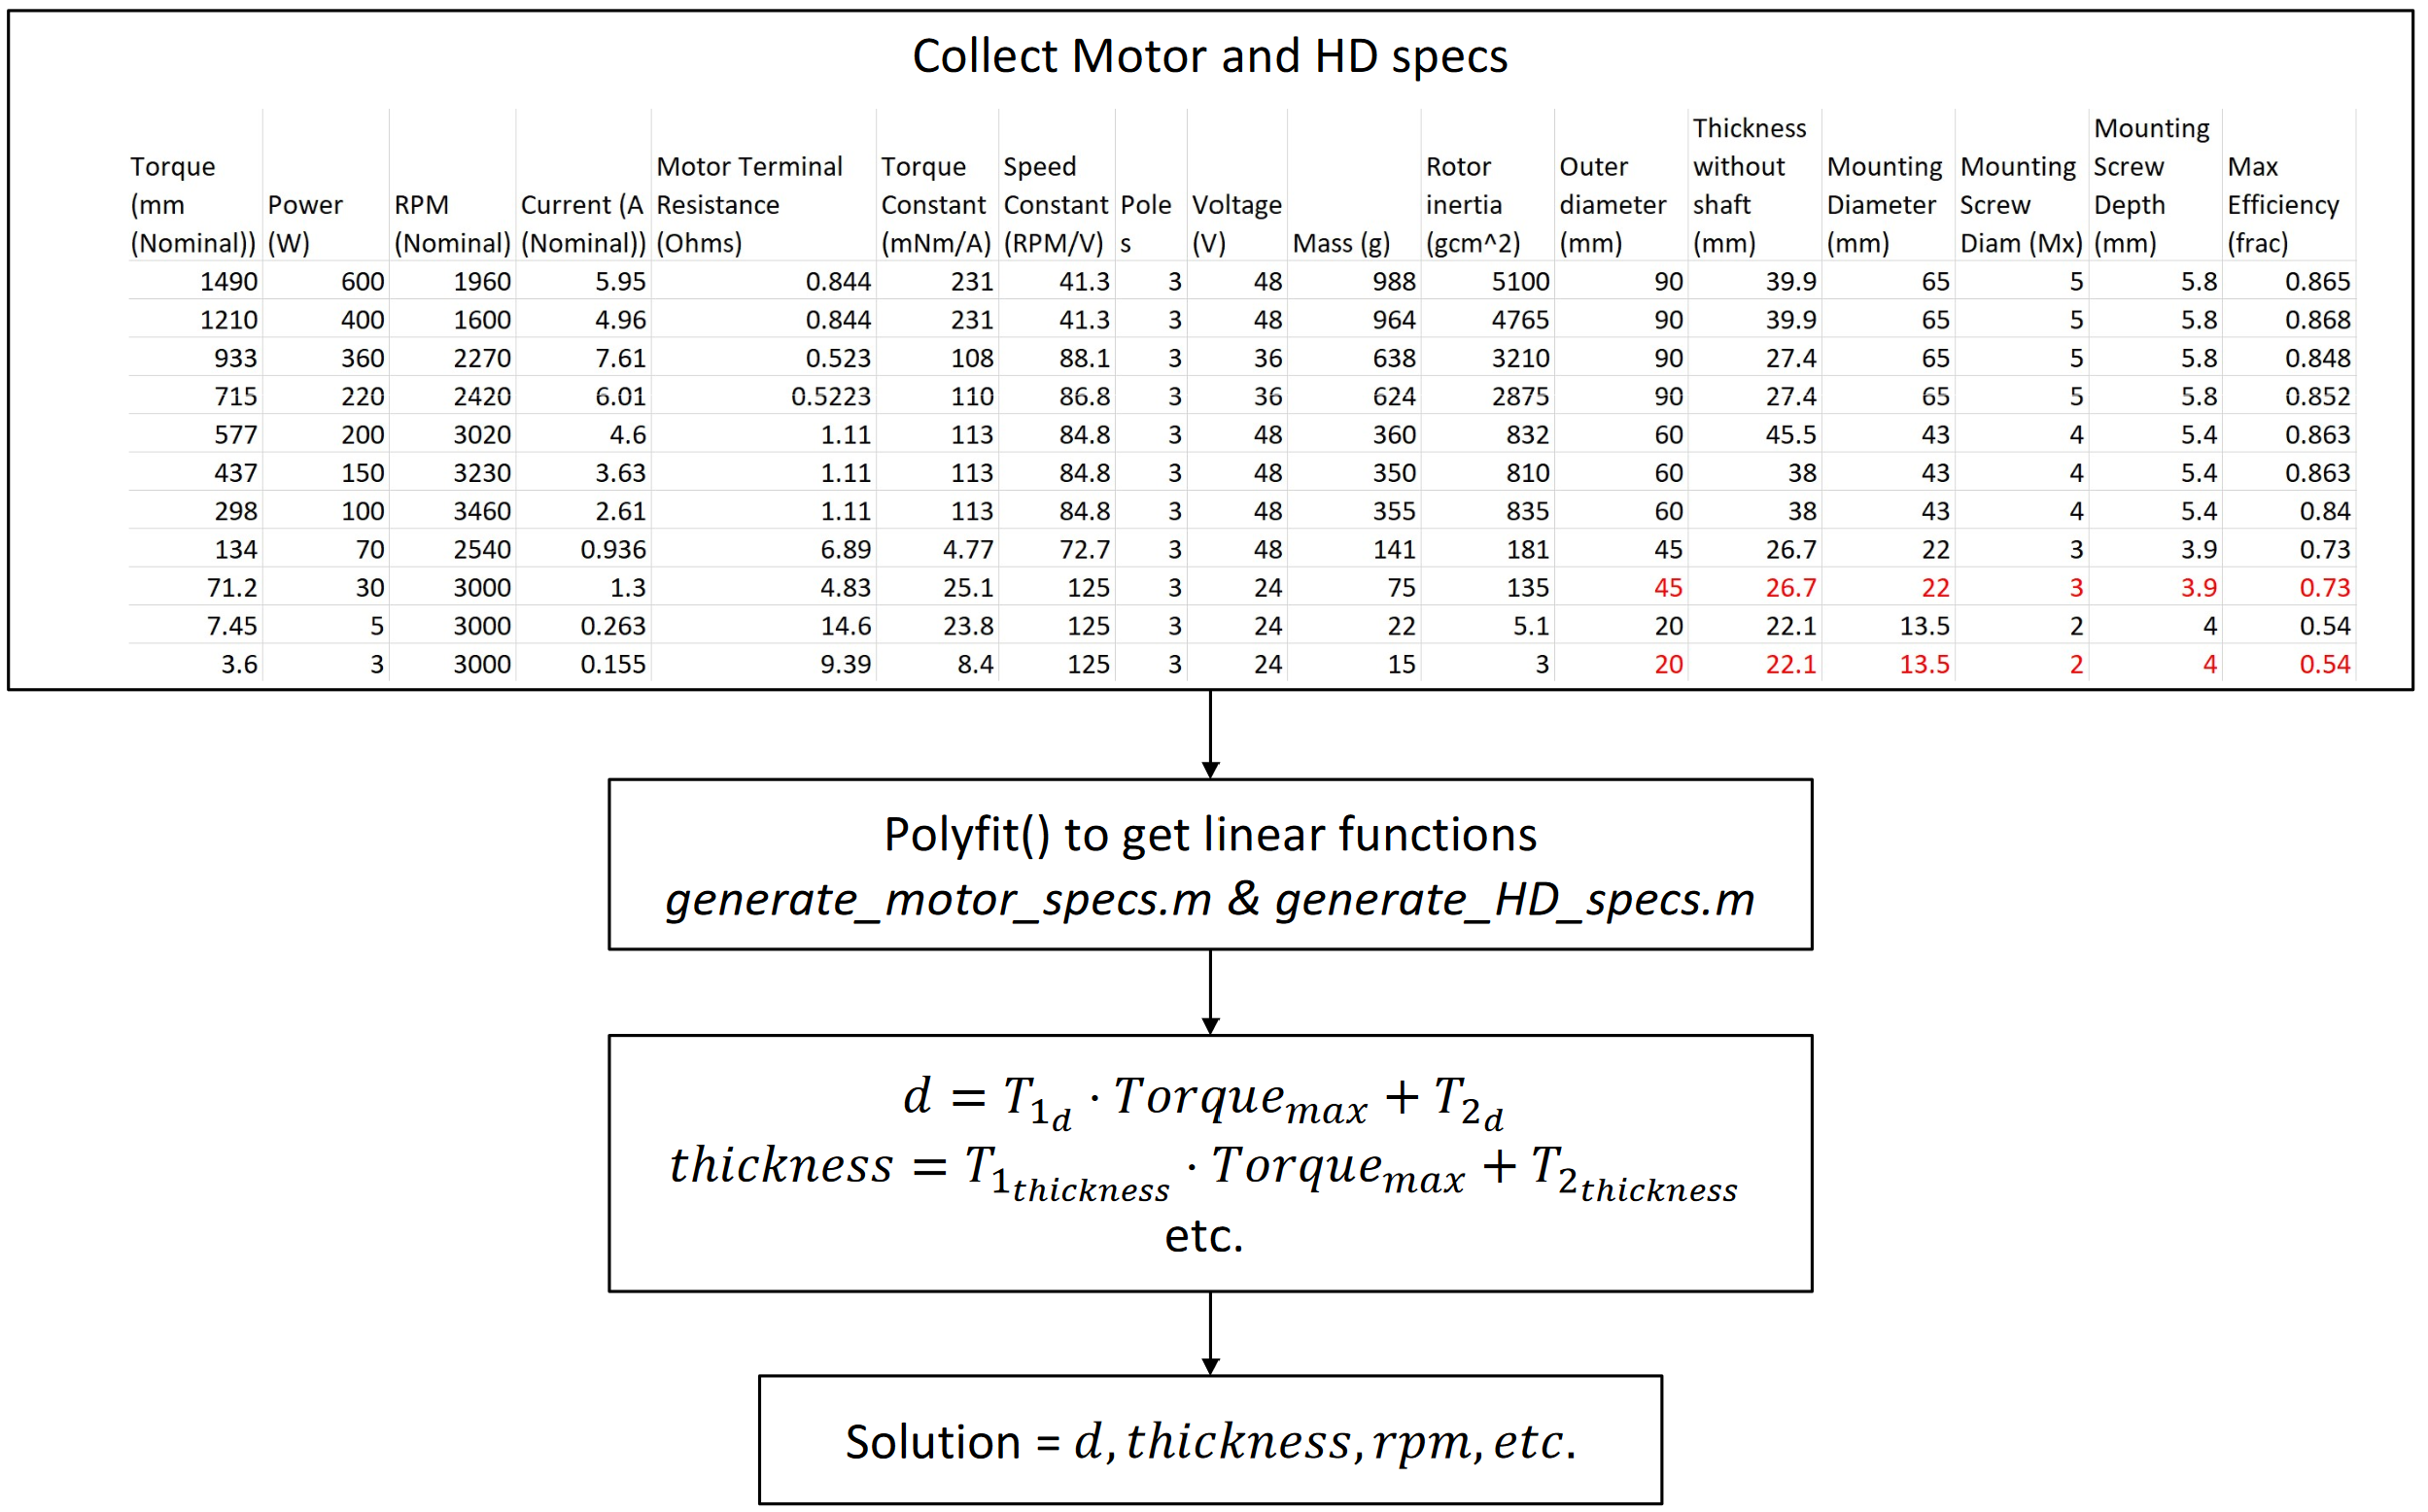
\includegraphics[width=\textwidth]{6_Appendices/Flowcharts/MotorAndHDFlowchart.png}
    \caption{Parameterization of Harmonic Drives and Motors}
    \label{fig:parametrization_HD_motor}
\end{figure}{}

%----------- VOLUMETRIC PARAMETRIZATION / VECTORIZATION -----------%
\subsection{Volumetric Parameterization and Vectorization} \label{app_sub:vectorization}

\subsubsection{Bolts} \label{app_ssub:vectorization_bolt}

All components but the springs and bolts were determined using the classic \texttt{for} loops found in Appendix \ref{app_sec:flowcharts}; all geometric variables are set as constants or ratios of a single parameterized variable.
The bolts employ a simple vectorized approach, where a range of bolt diameters is generated using \texttt{d = linspace(startval,endval,numberofsteps);}.
The regular stress and safety factor equations are vectorized, giving an array of safety factors for each diameter.
These can be filtered using \texttt{find(SF > 1.5, etc.)} to find all diameters matching certain conditions, and the final diameter is minimized by selecting the smallest amongst the matching diameters.
This procedure is demonstrated in Figure \ref{fig:vectorized_bolts}.

\begin{figure}[H]
    \centering
    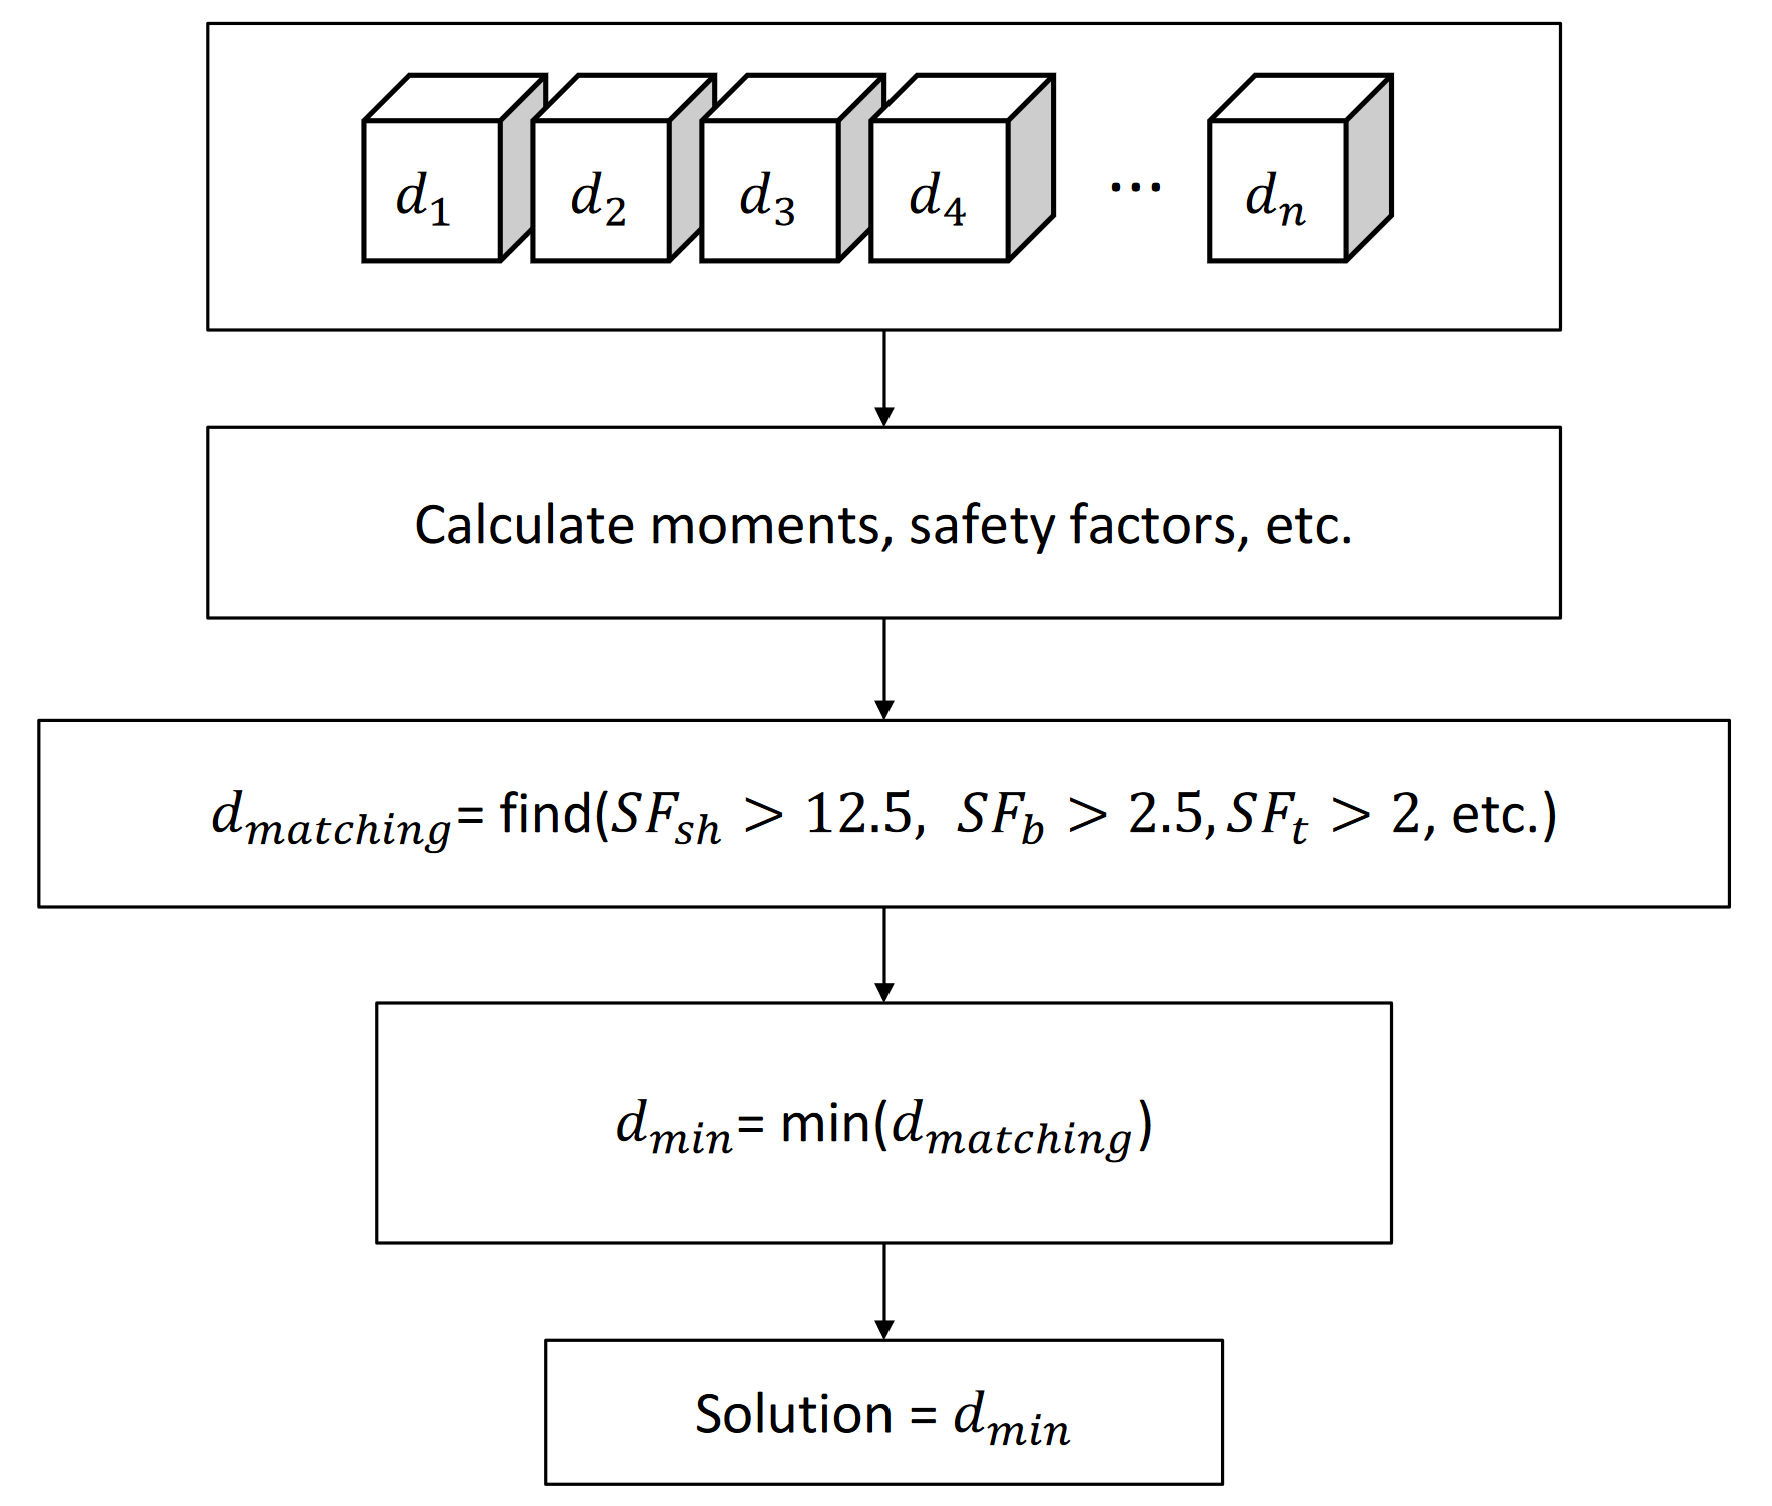
\includegraphics[width=\textwidth]{3_Parametrization/img/VectorizedBolts.png}
    \caption{Flowchart of vectorized bolts. Note how looping is not necessary and the time to find a solution is constant}
    \label{fig:vectorized_bolts}
\end{figure}{}

As well as computing the ideal solution in constant time and taking advantage of MATLAB's superior vectorization performance, this technique can easily be extended to multiple dimensions \cite{mathworks_vectorization_2019}.

\subsubsection{Springs} \label{app_ssub:vectorization_spring}

The spring has three primary parameters: the number of twists $N_f$, wire diameter $d$ and total diameter $D$.
All three can be expressed as row, column and depth vectors using \texttt{linspace()}, then duplicated into 3D matrices.
These are then passed through the stress analysis equations, and 3D matrices of safety factors and spring constants are found.
The same \texttt{find()} function can be used to find combinations meeting minimum safety factor and maximum diameter requirements, amongst others.
The ideal combinations is then selected by minimizing the total spring length $L = N_f \cdot d$.
The 3D procedure is demonstrated in Figure \ref{fig:vectorized_springs}.

\begin{figure}[H]
    \centering
    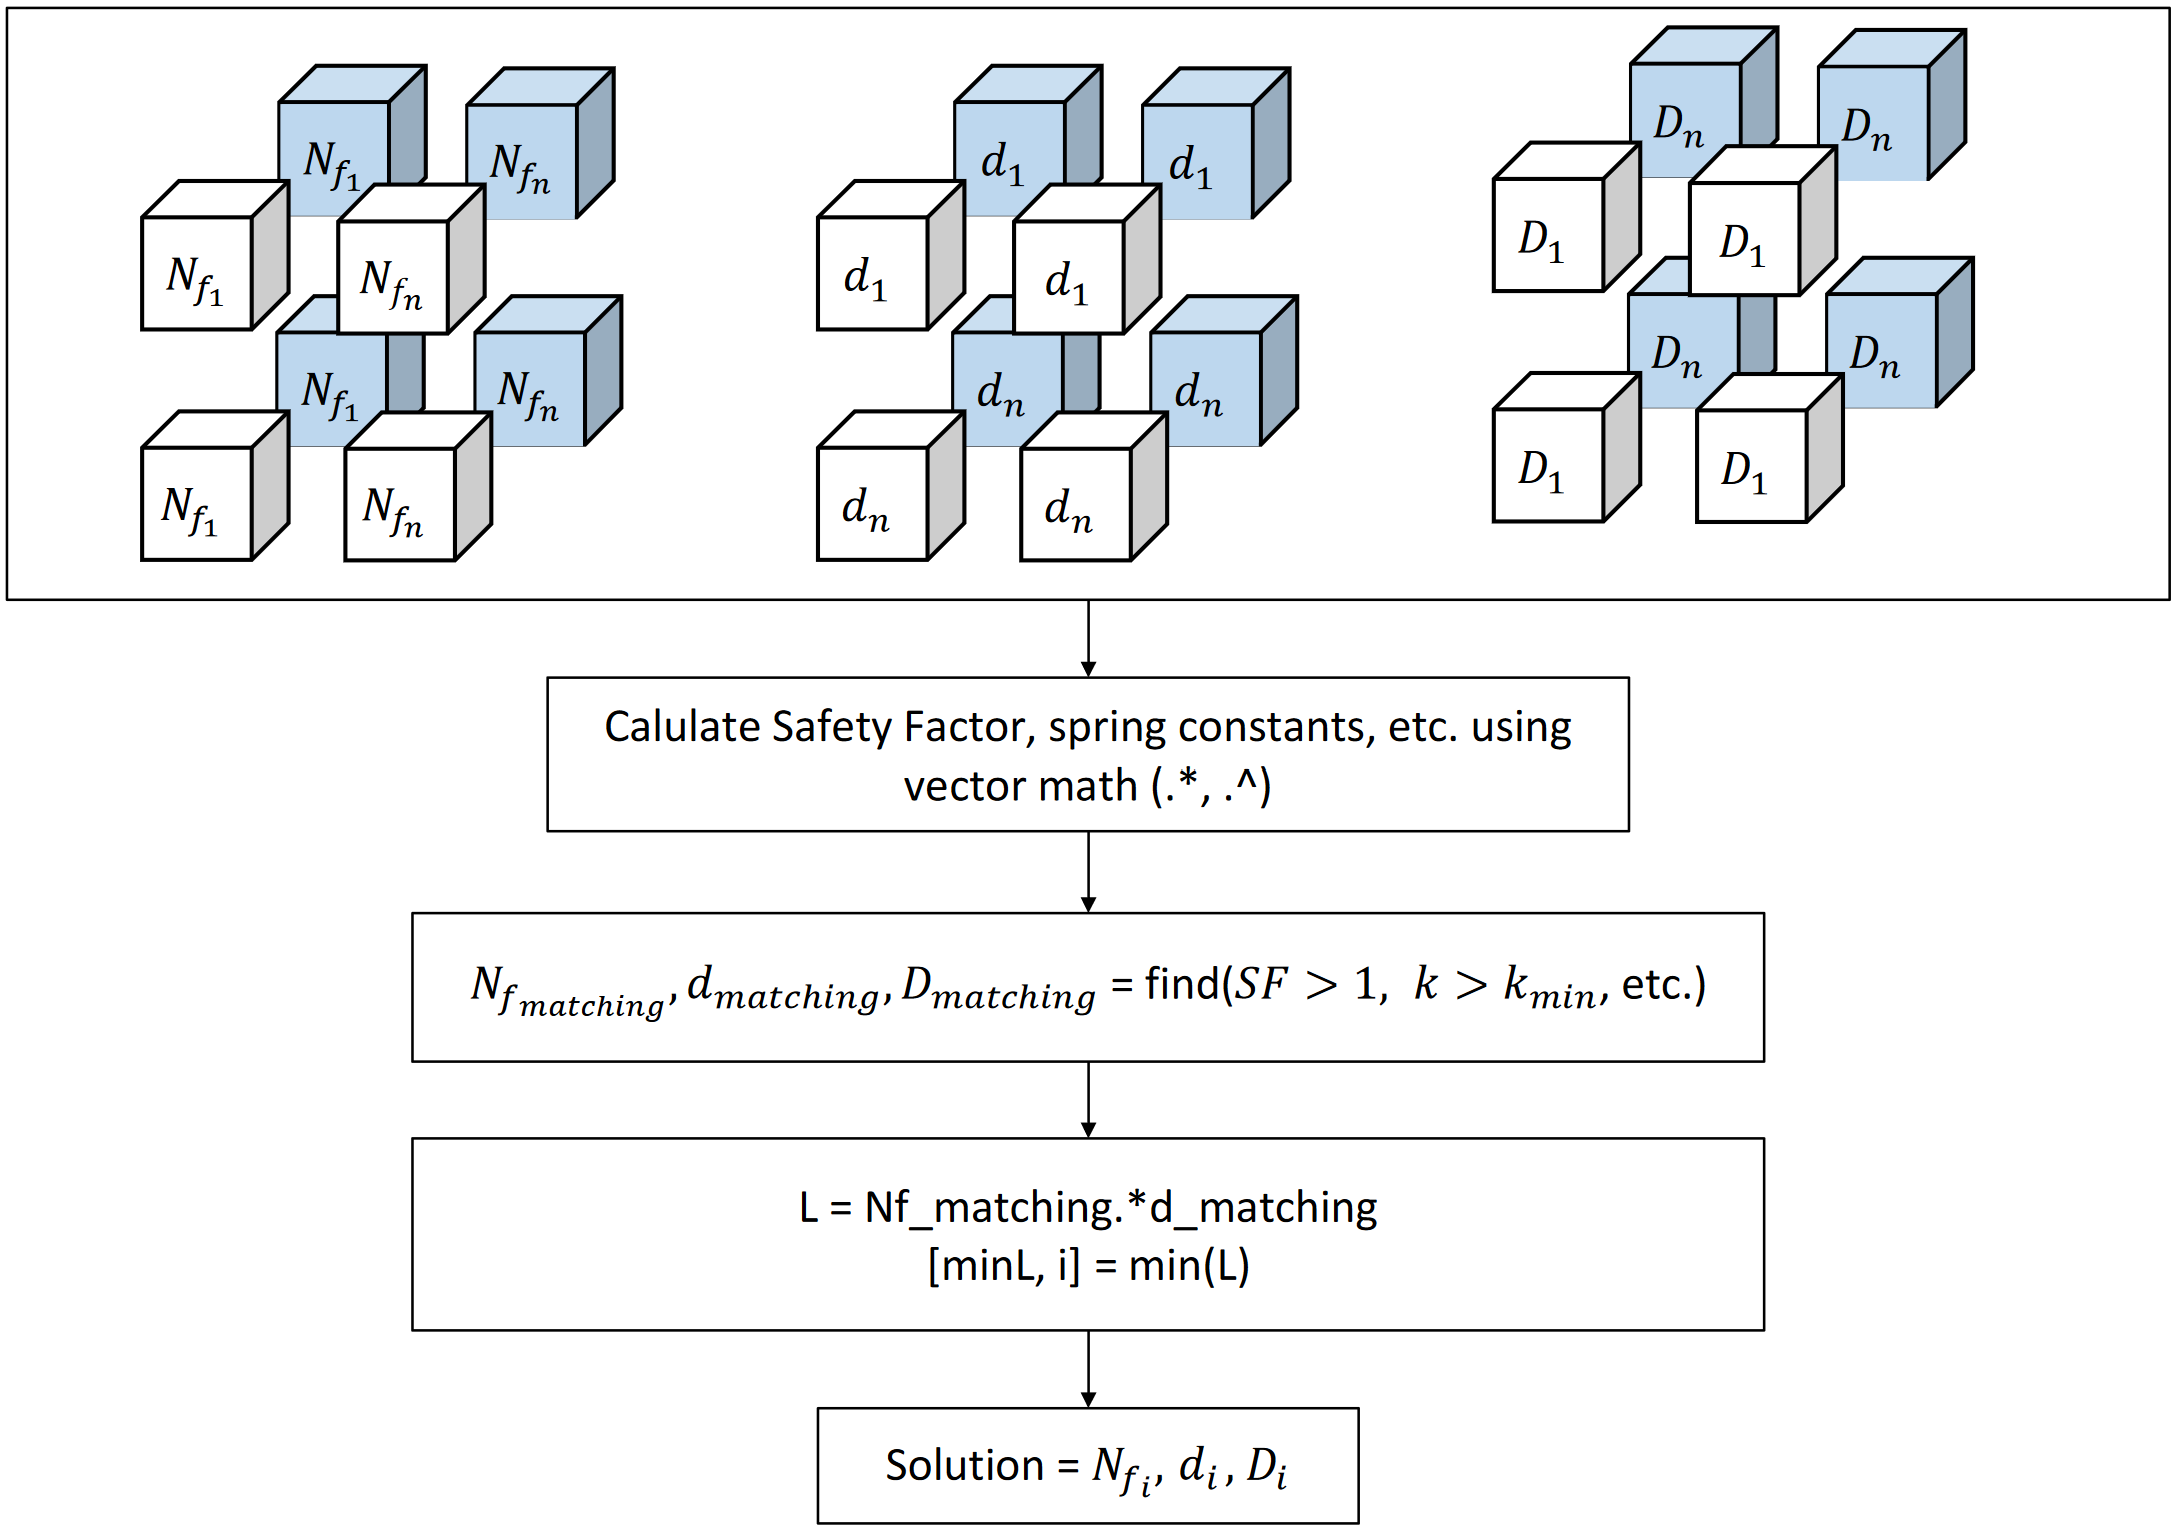
\includegraphics[width=\textwidth]{3_Parametrization/img/VectorizedSprings.png}
    \caption{Flowchart of vectorized springs. As with Figure \ref{fig:vectorized_bolts}, there is no looping required}
    \label{fig:vectorized_springs}
\end{figure}{}

The consequence of this method is a larger memory footprint, as large matrices must be stored.
It greatly simplifies the optimization procedure, is much more simple to implement than a gradient descent algorithm, and in hindsight could have been employed for parts where simplifications had to be made to reduce the optimization problem to one variable \cite{kathuria_intro_2018}.